\documentclass[grad,pdftex]{poli}
\usepackage[utf8]{inputenc}
\usepackage{amsmath,amssymb}

\makelosymbols
\makeloabbreviations

\begin{document}
  \title{Solução da equação transiente do calor através do método de elementos finitos aplicado a discos de freio}
  \foreigntitle{Solution of the transient heat equation using the finite element analysis applied to brake discs}
  \author{Felipe Rodrigues de Mello}{Alves}
  \advisor{Prof.}{Gustavo}{Rabello dos Anjos}{D.Sc.}
  \coadvisor{Prof.}{Gustavo Rabello}{dos Anjos}{D.Sc.}
  \examiner{Prof.}{Roney Leon Thompson}{D.Sc.}
  \examiner{Prof.}{Roney Leon Thompson}{Ph.D.}
  \examiner{Prof.}{Roney Leon Thompson}{D.Sc.}
  \department{DEM}
  \date{12}{2020}
  \keyword{Equação do calor}
  \keyword{Método de elementos finitos}
  \keyword{Discos de freio}
  \maketitle

  \frontmatter
  \dedication{À minha família por todo o suporte e compreensão.\\
}


  \chapter*{Agradecimentos}

Sou muito grato ao investimento financeiro e educacional fornecido pelos meus pais Eduardo e Isabel e o apoio da minha dinda Daize na formação profissional. Agradeço ao suporte de todos os meus amigos de fora da faculdade que perceberam meus momentos difíceis e foram capazes de me apoiar mesmo sem entender bem a realidade do curso e a meus amigos de faculdade que foram grandes companheiros em momentos de extrema importância. Um agradecimento enorme à equipe Icarus de Formula SAE por me proporcionar a paixão pela engenharia mecânica e me ensinar a ser um engenheiro mais completo. 



  \begin{abstract}

Este trabalho propõe o desenvolvimento de um código capaz de calcular soluções aproximadas para o problema térmico aplicado a discos de freio submetidos à situaçõoes críticas de frenagem de um protótipo de competição tipo formula utilizando o método de elementos finitos. A solução da equação transiente de calor aplicada a um disco de freios fornece uma alternativa aos softwares de altos investimentos financeiros e capacidades computacionais no momento do estudo da dissipação de calor, resultando em um parâmetro de escolha de materiais para fabricação e geometrias a serem consideradas.

\end{abstract}


  \begin{foreignabstract}

Eigenvalues and eigenvectors of linear operators are important in many Applied
Mathematics areas. In Civil Engineering, especially in Structural Analysis,
eigensystems have a fundamental importance. A typical example is in dynamic
analysis, where the eigenvalues represent the natural frequencies and
eigenvectors the mode shape. The increasing demand for efficient numeric
evaluation of eigenvalues and eigenvectors motivated the search for new methods
for the solution of complex eigensystems.

\end{foreignabstract}


  \tableofcontents
  \listoffigures
  \listoftables
  \printlosymbols
  \printloabbreviations

  \mainmatter
  \chapter{Introdução}

Para transformar um problema real em um modelo compatível com soluções computacionais existem algumas metodologias de idealização do fenômeno físico - onde traduzimos suas características através de modelos matemáticos - a fim de discretizá-lo e resolvê-lo, como esquematizado na Figura \ref{fig:modelos}.

\begin{figure}[hb]
\centering
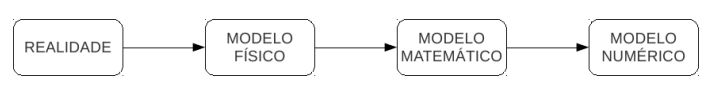
\includegraphics[scale=0.7]{Imagens/Modelos}
\caption{Modelagem de problemas reais para solução numérica}
{\footnotesize Fonte: Elaborada pelo autor.}
\label{fig:modelos}
\end{figure}

As simulações computacionais fazem uso de diferentes métodos e técnicas para calcular soluções envolvendo os problemas típicos da ciência e engenharia, como: método de diferenças finitas, método de elementos finitos e método de volumes finitos. O método dos elementos finitos (MEF) é um procedimento que busca soluções aproximadas para os modelos numéricos e se aplica a uma grande variedade de problemas físicos. Sua acurácia e estabilidade estão largamente estudados, o que confere ao método uma robustez e sólida confiabilidade.

Para viabilizar a solução, a modelagem divide uma geometria grande e complexa, que é submetida a carregamentos térmicos ou mecânicos em pequenas partes – denominadas \textit{elementos} - os quais passam a representar o domínio contínuo do problema. A filosofia por trás do método é reduzir um problema grande (seu objeto de estudo) em problemas menores (os \textit{elementos}) e calcular também a relação entre eles. O conjunto dos \textit{elementos} e de seus pontos de contorno – denominados nós – é conhecido como \textit{malha}. A \textit{malha}, portanto, é composta por um número finito de \textit{elementos} de comportamento bem definido. O método de elementos finitos é um método poderoso para discretizaçãoo de geometrias complexas pois não exige esforço adicional comparado a sua utilização em geometrias regulares. 
 
A precisão do método dos elementos finitos (MEF) depende da quantidade de nós e elementos, do tamanho e dos tipos de elementos da malha. Ou seja, quanto menor for o tamanho e maior for o número dos elementos em uma determinada malha, maior a precisão nos resultados da análise.

\section{Motivaç{\~ a}o}
Veículos de competição são submetidos a grandes esforços uma vez que o seu objetivo é ser mais eficaz em uma pista de corrida. As pistas planejadas para veículos de alta performance são compostas de diversos trechos curvos, principalmente as pistas de Formula SAE e a frenagem eficiente permite maior precisão nas entradas de curva. Sendo assim o sistema de freios é constantemente acionado, o que leva a um considerável aumento de temperatura dos seus componentes. O aumento descontrolado de temperatura nos discos de freio podem resultar em fadiga, vaporização do fluido de freio, rachaduras térmicas e vibrações prejudiciais ao funcionamento do sistema, o que compromete a segurança e performance do protótipo.

\section{Objetivo}
Estudar os fenômenos energéticos envolvendo os componentes dos freios e apresentar soluções computaconais a fim de proporcionar comparativos das influências das grandezas envolvidas no projeto.

\section{Metodologia}

\section{Organizaç{\~ a}o da tese}

  \chapter{Revisão Bibliográfica}

Em um disco de freios ocorrem os três tipos de transferência de calor descrito por  Frank P. Incropera ~\cite{Lan50a}: condução, convecção e radiação. O autor define transferência de calor como energia térmica em trânsito devido a uma diferença de temperatura no espaço. Quando existe um gradiente de temperatura em um meio estacionário sólido ou fluido a condução ocorre quando há transferência de calor através do meio. Já a convecção ocorre quando há trasferência de calor entre uma superfície e um fluido em movimento. Quando a troca de calor ocorre através de ondas eletromagnéticas que são emitidas por qualquer superfície com temperatura não nula, ocorre a radiação. O estudo desses fenômenos ocorre através de equações de taxas que quantificam a energia transferida por unidade de tempo.

A condução pode ser interpretada como um fenômeno difusivo onde ocorre transferência de energia das partículas mais energéticas para as menos energéticas através das interações entre partículas. Em um sólido essas interações ocorrem através da combinação entre a vibração das moléculas dos retículos cristalinos e a movimentação dos elétrons livres. Para a condução a equação que descreve a taxa de transferência de calor é conhecida como a \textit{lei de Fourier}.

$$ \textbf{q} = -k \nabla \textbf{T} = -k \left(\textbf{i} \frac{dT}{dx} + \textbf{j} \frac{dT}{dy} + \textbf{k} \frac{dT}{dz} \right) $$

sendo $\textbf{q}$ o fluxo de calor e $k$ a condutividade térmica.



Denotemos o domínio por $\Omega$\symbl{$\Omega$}{domínio de definição de uma
equação diferencial}. Seja $\partial \Omega$ o contorno de
$\Omega$.\symbl{$\partial$}{operador do contorno.}

\begin{equation}
	|x| = \left\{ \begin{array}{ll}
	1 & \mbox{, se } x \geq 0; \\
	-1 & \mbox{, se } x < 0. \end{array} \right.
\end{equation}


  \chapter{Método Proposto}

\section{O Algoritmo}
Vamo fazer um teste.

\begin{figure}[hb]
\centering
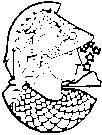
\includegraphics{Imagens/minerva}
\caption{Deusa Minerva.}
\label{fig:minerva}
\end{figure}

Isso foi um teste.
  \chapter{Resultados e Discussões}

\section{Metodologia para avaliaç{\~ a}o do M{\' e}todo}

\section{Validaç{\~ a}o da rotina implementada}

\subsection{Problema de autovalor padr{\~ a}o -- Caso I}

A Tabela~\ref{table:casoi} mostra as variações dos parâmetros escolhidos para
análise.

\begin{table}[hb]
\caption{Par{\^ a}metros do teste realizado com a matriz de Wilkinson,
3 autovalores computados.}
\label{table:casoi}
\centering
\begin{tabular}{cccc}
  \hline
  TValor de ``m'' & N$^{o}$ de iteraç{\~ o}es & Tempo de CPU & Norma do Res{\' i}duo\\
  \hline
  6 & 100 & 0,09013 & $7,1474 \times 10^{-12}$\\
  10 & 28 & 0,09025 & $1,5387 \times 10^{-13}$\\
  20 & 10 & 0,100144 & $5,9011 \times 10^{-14}$\\
  40 & 6 & 0,16022 & $8,67438 \times 10^{-14}$\\
  50 & 3 & 0,24034 & $1,51537 \times 10^{-15}$\\
  \hline
\end{tabular}
\end{table}

  \chapter{Conclusões}


  \backmatter
  \nocite{*}
  \bibliographystyle{poli-unsrt.bst}
  \bibliography{thesis}
  \appendix
  \chapter{Código Fonte}

\end{document}
